
% part 1
\section{С чего мы начнем вначале\label{sec:part1}}



    Данная статья является переводом. Оригинал, который можно найти на странице  
\href{http://krondo.com/?page\_id=1327}{Twisted Introduction},
был написан Dave Peticolas.


\subsection{Предисловие}


    В рассылке Twisted не так давно появился вопрос:  
можно ли где-нибудь найти описание, которое 
позволит быстро овладеть техникой использования Twisted? 
На данный момент такого описания не существует, и данное 
руководство им не является.


Если вы новичок в асинхронном программировании, то  
лучше изучать основные принципы постепенно. 
Исходя из продолжительного опыта использования Twisted и 
познания всех тонкостей и сложностей, данное пособие начинается с 
общего понятия модели асинхронного программирования. 
Большая часть кода Twisted понятна и 
хорошо написана, документация на сайте хорошая, по меньшей 
мере с точки зрения стандартов свободного ПО. Но без понятия модели, 
чтение кода Twisted или кода, использующего Twisted, или даже чтение 
документации, превратится в головную боль.


Таким образом, первые главы помогают 
осознать модель асинхронного программирования, а последующие - 
постичь особенности программирования с использованием Twisted. 
В самом начале мы совсем не будем использовать Twisted. 
Вместо этого, для иллюстрации функционирования асинхронной системы 
мы будем использовать простые программы на Python'е. И как только мы 
начнем использовать Twisted, мы начнем с очень низкого уровня, который 
вы не использовали бы в повседневном программировании. Twisted - 
высоко абстрактная система, и это дает вам огромное преимущество при решении 
проблем. Но, когда вы изучаете Twisted, в особенности, когда вы 
пытаетесь понять как Twisted реально работает, многоуровневые абстракции могут 
быть препятствием. Поэтому мы начнем с самых основ.


После того, как вы осознаете модель, вам будет проще 
читать документацию и исходный код Twisted. Так что - начнем. 


\subsection{Модели}


    Мы начнем с рассмотрения двух похожих моделей,
для того чтобы сравнить с ними асинхронную модель.
Для иллюстрации мы представим программу, которая
состоит из трех концептуально отличных задач,
которые должны быть выполнены, для того чтобы программа
завершилась. Мы конкретизируем эти задачи позже, сейчас
мы не будем говорить ничего о них, кроме того, что программа
должна выполнить эти задачи. Заметьте, что термин ``задача'' 
используется не в техническом смысле: ``нечто, что нужно выполнить''.



Первая модель, которую мы рассмотрим, - однопоточная синхронная модель, изображенная 
на рисунке \ref{fig:sync} ниже:

% fig1
\begin{figure}[h]
\begin{center}
    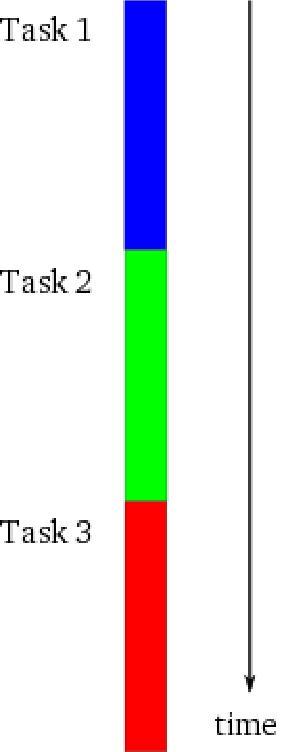
\includegraphics[height=0.3\textheight]{images/sync.pdf}
\end{center}
    \caption{Синхронная модель\label{fig:sync}}
\end{figure}

Это самый простой стиль программирования. Одновременно выполняется только одна задача, 
следующая задача выполняется только после того, как предыдущая завершилась. И, если 
задачи всегда выполняются в определенном порядке, то запуск следующей задачи 
может осуществиться, если все предыдущие задачи завершились без ошибок.


Мы можем сравнить синхронную модель с многопоточной моделью, изображенной 
на рисунке \ref{fig:threaded}:

% fig2
\begin{figure}[h]
\begin{center}
    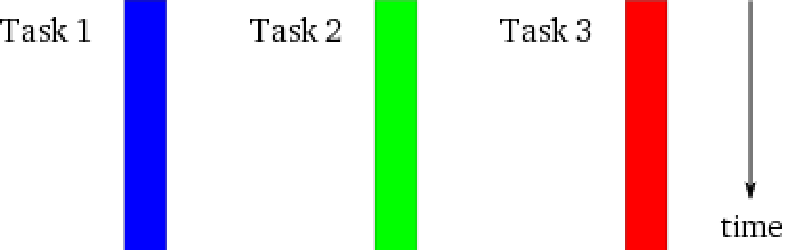
\includegraphics[width=0.5\textwidth]{images/threaded.pdf}
\end{center}
    \caption{Модель на основе потоков\label{fig:threaded}}
\end{figure}

В этой модели каждая задача выполняется в
отдельном потоке. Потоки управляются операционной системой, и в
случае наличия нескольких процессоров и/или ядер, 
могут выполняться параллельно, или их выполнение
может чередоваться в случае одного процессора. Смысл в том, что
в тредовой модели деталями управляет операционная система, и 
программист просто думает в терминах независимых потоков инструкций,
которые могут выполняться одновременно. Хотя диаграмма простая, на
практике потоковые программы могут быть достаточно сложными,
поскольку нужно координировать потоки между собой. Потоковая координация и
взаимодействие являются отдельной, достаточно сложной темой.

Некоторые программы реализуют параллельность, используя несколько
процессов вместо нескольких потоков. Хотя, с точки зрения реализации есть
отличия, для наших целей это одна и та же модель, как на рисунке \ref{fig:threaded}.


Теперь мы можем перейти к асинхронной модели на рисунке \ref{fig:async}:

% fig3
\begin{figure}[h]
\begin{center}
    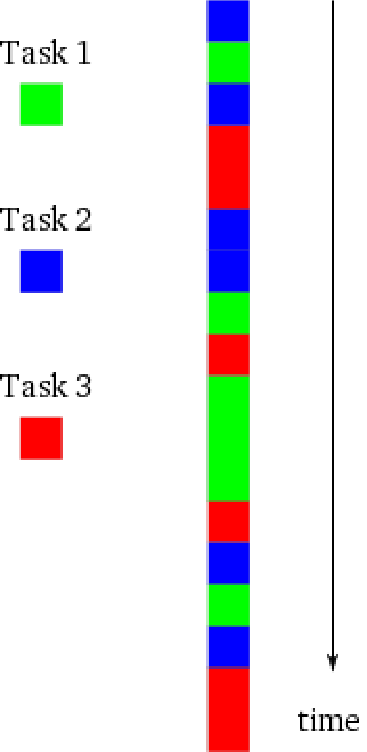
\includegraphics[height=0.3\textheight]{images/async.pdf}
\end{center}
    \caption{Acинхронная модель\label{fig:async}}
\end{figure}

В этой модели задачи выполняются поочередно в одном потоке. 
Это проще, чем в случае потоков, поскольку программист всегда знает, что
когда одна задача выполняется, другая - нет. Хотя в однопроцессорной системе
в потоковой программе задачи также будут выполняться поочередно, программист,
использующий потоки, все равно должен думать в терминах рисунка \ref{fig:threaded},
а не \ref{fig:async}, чтобы программа работала корректно при переходе
на многопроцессорную систему. Но однопоточная асинхронная система всегда
будет чередовать выполнение задач даже на многопроцессорной системе.


Существует еще одно отличие между асинхронной и потоковой моделями.
В потоковой модели решение приостановить один поток и выполнить другой
в большей степени не регулируется программистом. Скорее, это контролируется
операционной системой, и программист должен предполагать, что поток
может приостановиться и смениться другим практически в любой момент времени.
Что отличается от задач в асинхронной модели, которые выполняются до того момента,
когда явно не передают контроль другим задачам. Это значительно проще, чем
в случае потоков.


Заметим, что возможно смешивать асинхронные и потоковые модели, и использовать
оба варианта в одной системе. Но, для большей части этого введения,
мы будем придерживаться ``чистых`` асинхронных систем с управлением в один поток.


\subsection{Мотивация}


    Мы увидели, что асинхронная модель проще, чем потоковая, поскольку 
есть только единственный поток инструкций и задач, который явно передает 
управление, вместо приостановки в произвольный момент времени. Но 
асинхронная модель является явно более сложной, чем синхронная. 


Программист должен организовать задачу как последовательность 
маленьких шагов, которые периодически запускаются.


И, если одна задача использует вывод другой, то зависящая 
задача должна быть написана так, чтобы уметь принимать на вход  
результат по порциям, вместо одного большого куска.


Поскольку здесь нет параллельности, что видно из 
наших диаграмм, то асинхронная программа будет 
выполняться также долго как и синхронная, возможно дольше, 
так как асинхронная программа может быть
хуже с точки зрения локальности ссылок.


Так почему же мы бы выбрали асинхронную модель? 
Существует по меньшей мере две причины. 
Первая - если одна или более задач отвечают за реализацию интерфейса, 
то путем чередования задач, система сможет отвечать 
на пользовательский ввод даже тогда, когда в ``фоне'' выполняется 
другая задача. Так как фоновые задачи не могут выполниться быстрее, 
система будет более вежливой для того, кто ее использует. 
Однако, существуют условия, когда асинхронная система 
будет лучше по сравнению с синхронной, иногда намного, в смысле 
выполнения всех задач за более короткий промежуток времени.
Эти условия связаны с задачами, которые вынуждены ожидать событий 
или блокироваться, как это изображено на рисунке \ref{fig:block}: 

% fig4
\begin{figure}[h]
\begin{center}
    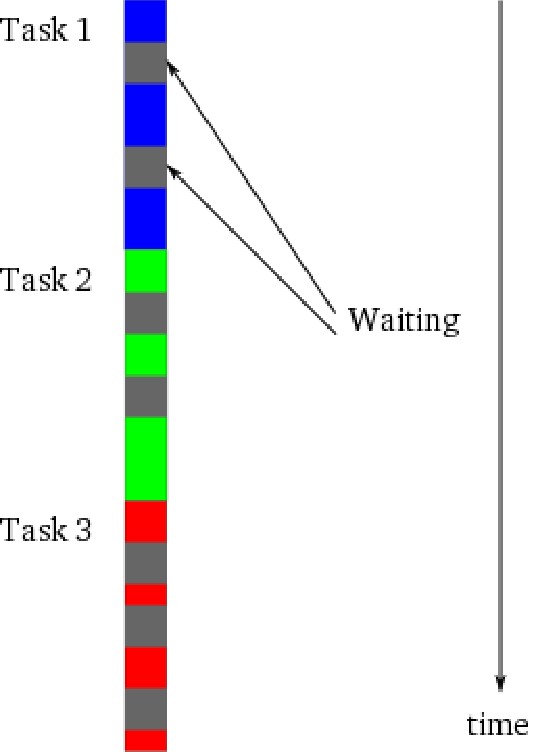
\includegraphics[height=0.3\textheight]{images/block.pdf}
\end{center}
    \caption{Блокирование в синхронной программе\label{fig:block}}
\end{figure}

На рисунке серые секции представляют собой периоды времени, 
когда определенная задача ожидает (блокируется) и не выполняется. 
Почему же задача может быть заблокирована? Частая причина - ожидание 
выполнения  ввода-вывода, связанное с перенесением 
данных из или во внешнее устройство. Обычный процессор может 
управлять переносом данных на порядок быстрее, по сравнению с максимальной 
скоростью переноса данных для диска или сети. Таким образом, синхронная 
программа, которая выполняет много операций ввода-вывода, будет 
часто блокироваться в момент обращения к диску или сети. Такая синхронная 
программа часто называется блокирующаяся программа (blocking program).


Заметьте, что на рисунке \ref{fig:block} изображена блокирующаяся программа, 
которая немного похожа на асинхронную программу на рисунке \ref{fig:async}. 
Это не совпадение. Основная идея в асинхронной модели - это то, что, когда  
асинхронная программа сталкивается с тем, что блокирует синхронную 
программу, асинхронная будет выполняться. Асинхронная программа будет 
``блокироваться'' только тогда, когда нет задач на выполнение, поэтому 
такая программа называется неблокирующейся (non-blocking program). 
И каждое переключение с одной задачи на другую соответствует тому, что 
первая задача или выполнилась, или находится в месте, где она заблокирована. 
С большим количеством потенциально блокирующихся задач, 
асинхронная программа может превосходить синхронную тем, что проводит 
в целом меньше времени ожидая.


По сравнению с синхронной моделью, асинхронная модель лучше когда:

\begin{enumerate}

\item Когда есть много задач таких, что почти всегда есть по меньшей мере 
    одна задача, которая может выполняться.
\item Задачи выполняют много операций ввода-вывода, приводя к тому, что
    синхронная задача проводит много времени впустую, блокируясь, в то время 
    когда другие задачи могли бы выполняться.
\item Задачи независимы друг от друга и не нуждаются во 
    взаимодействии.
\end{enumerate}


Эти условия почти полностью характеризуют типичный сетевой сервер (например, 
web сервер) в среде клиент-сервер. Каждая задача представляет собой один 
клиентский запрос с операциями ввода-вывода в форме получения запроса и 
отправления ответа. И клиентские запросы по большому счету независимы. 
Так что реализация сетевого сервера является подходящим кандидатом для 
асинхронной модели, поэтому Twisted - это одна из первых и передовых 
сетевых библиотек. 


\subsection{Дальше и больше}


    Это окончание первой части. Во второй части мы будем писать 
некоторые сетевые программы, обе - блокирующиеся и неблокирующиеся, 
настолько простые, насколько это возможно (без использования Twisted), 
для того, чтобы осознать как действительно работает 
асинхронная программа, написанная на Python'е.


